% !TeX spellcheck = it_IT
\newpage
\section{Green Computing}
In generale, il green computing può aiutare le organizzazioni a ridurre l'impatto ambientale e a risparmiare sui costi energetici e di gestione.

\begin{definition}[Green Computing]
	Il green computing tratta la \textbf{progettazione}, la \textbf{realizzazione} e l'\textbf{utilizzo} di \underline{sistemi ICT}, \underline{computer} e \underline{dispositivi elettronici}\footnote{Tutti quei dispositivi che si appoggiano all'informatica per funzionare, e.g. aspirapolvere} in modo responsabile e sostenibile dal punto di vista ambientale, considerando in particolare il \textbf{consumo energetico} e \textbf{impronta di carbonio}.
\end{definition}

\begin{definition}[$CO_2$-eq]
	L'anidride carbonica equivalente è una misura che esprime l'impatto di una certa quantità di gas serra rispetto alla stessa quantità di anidride carbonica.
\end{definition}

\begin{definition}{Energy Star}
	Il progetto Energy Star nasce negli anni '90 ed è stata una delle prime iniziative relative al green computing per dare un indicatore dell'efficienza energetica. Il problema principale è che è \textbf{facoltativo}.
\end{definition}

\subsection{Approccio olistico}
Per funzionare segue un approccio \textbf{olistico}, analizzando tutto il \textbf{ciclo di vita} di un sistema, sia \emph{vericalmente} che \emph{orizzontalmente}.

\begin{itemize}
	\item \textbf{Progetto}: progettare in modo sostenibile computer, server, sistemi di raffreddamento e software a basso consumo e alta efficienza.
	\item \textbf{Produzione}: attenzione a non sprecare risorse limitate, ridurre gli scarti di fabbricazione e utilizzare fonti rinnovabili per la produzione.
	\item \textbf{Trasporto}: cercare di ridurre e ammortizzare l'uso di carburanti fossili sostituendoli con veicoli elettrici o ibridi e facendo spedizioni accorpate.
	\item \textbf{Uso}: utilizzare i sistemi cercando di ridurre il consumo con politiche di risparmio (e.g. ibernazione)
	\item \textbf{Dismissione}: lo smaltimento di dispositivi elettronici attraverso il riciclo
\end{itemize}

\subsection{Pilastri fondamentali}
\begin{center}
	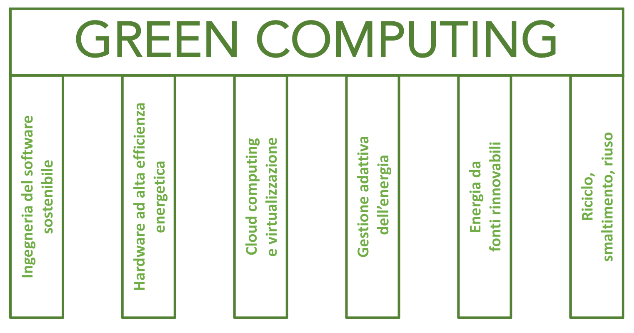
\includegraphics[scale=0.5]{green_pilastri.png}
\end{center}
\subsubsection{Ingegneria del software sostenibile}
È possibile fare in modo che i programmi consumino meno energia e che il loro dispiegamento nelle varie fasi del ciclo di vita produca minori gas inquinanti. In particolare, programmare \emph{sfruttando le peculiarità di linguaggi e hardware} che possano rendere il software più disponibile.
\subsubsection{Hardware ad alta efficienza energetica}
\subsubsection{Cloud computing e virtualizzazione}
\subsubsection{Gestione adattiva dell'energia}
\subsubsection{Energia da fonti rinnovabili}
\subsubsection{Riciclo, smaltimento, riuso}
È possibile \textbf{sensibilizzare} l'utente sul giusto uso dei mezzi a sua disposizione e quindi della loro conseguente fine di utilizzo. Ottimizzare l'impiego dei dispositivi porta una determinante longevità, minimizzando quindi il rifiuto.
\begin{itemize}
	\item Inoltre, per ridurre la produzione di rifiuti è fondamentale \textbf{riutilizzare} (ad esempio rivendendo) i dispositivi elettronici ancora validi. In molti casi è sufficiente sostituire componenti degradati (e.g. le batterie) e mantenere il resto. Oltretutto molti dispositivi possono essere considerati obsoleti per certi scopi ma ancora ottimi per altri (e.g. server).
	\item È fondamentale ingegnerizzare il processo di \textbf{smaltimento} in modo da permettere il \textbf{riciclo} di parte dei componenti. Ad esempio dalle schede stampate si possono recuperare metalli preziosi come l'oro. La legislazione italiana necessita il corretto trattamento dei rifiuti per ridurre l'inquinamento. Di conseguenza anche la scelta di macchinari e strumenti mirati allo smaltimento è fondamentale per fare in modo che un'azienda possa essere ritenuta green.
	\item La tecnologia stessa può essere uno strumento potente per \textbf{sensibilizzare} il consumatore su queste tematiche e per fargli conoscere le aziende green.
\end{itemize}
\subsection{Applicazioni green}
Sfruttare i sistemi ICT per l'\textbf{ottimizzazione} di processi che sfruttano risorse limitate (e.g. combustibili fossili nel trasporto, energia elettrica nel riscaldamento, acqua potabile nell'irrigazione) è un aspetto importante del green computing.